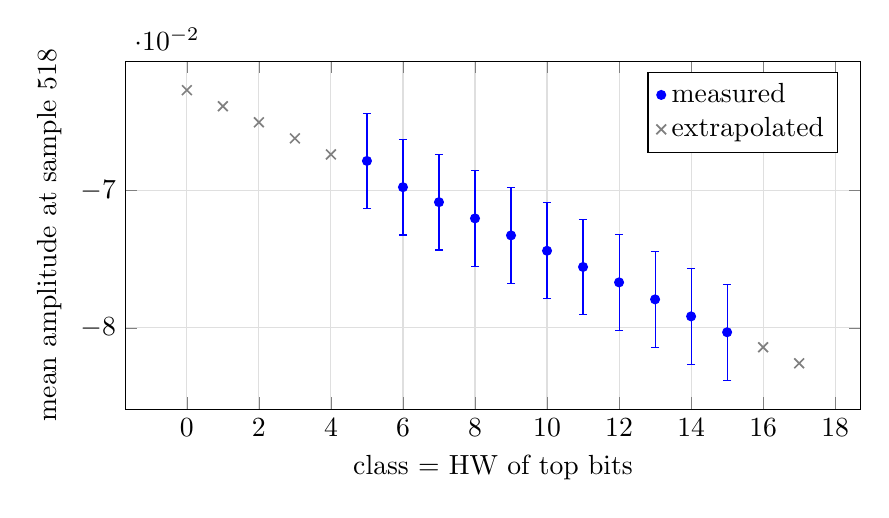
\begin{tikzpicture}
\begin{axis}[
  xlabel={class = HW of top bits},
  ylabel={mean amplitude at sample 518},
  width=0.9\linewidth,
  height=6cm,
  grid=major,
  grid style={gray!25},
  legend pos=north east,
  legend cell align=left,
]
\addplot[blue, semithick, mark=*, mark size=1.5pt, only marks, error bars/.cd, y dir=both, y explicit, error bar style={blue}] coordinates {(5,-0.0678424) +- (0,0.00348543) (6,-0.0697528) +- (0,0.00348543) (7,-0.0708448) +- (0,0.00348543) (8,-0.0720261) +- (0,0.00348543) (9,-0.0732637) +- (0,0.00348543) (10,-0.0743833) +- (0,0.00348543) (11,-0.0755624) +- (0,0.00348543) (12,-0.0766849) +- (0,0.00348543) (13,-0.0779216) +- (0,0.00348543) (14,-0.0791605) +- (0,0.00348543) (15,-0.0803153) +- (0,0.00348543)};
\addlegendentry{measured}
\addplot[gray, semithick, mark=x, mark size=2.5pt, only marks] coordinates {(0,-0.062691) (1,-0.0638608) (2,-0.0650307) (3,-0.0662005) (4,-0.0673703) (16,-0.0814084) (17,-0.0825783)};
\addlegendentry{extrapolated}
\end{axis}
\end{tikzpicture}
